\begin{multicols}{3}[\section{SIGFOX}]

\rhead{Sven Guthe}
\lfoot{18.05.2016}

\newrefsegment

\begin{tabular}{p{2,1 cm}p{2.7 cm}}
\textbf{Steckbrief}& \\
\end{tabular}
\rowcolors{1}{\topicolor!20}{}
\begin{tabular}{p{2,1 cm}p{2.7 cm}}
      Einsatz seit & Juni 2012\\
      Frequenz"-bereich  & \SI{868}{\mega\hertz} in der EU, \SI{915}{\mega\hertz} in den US\\
      Datenrate & bis zu \SI{100}{byte/s}\\
      Verbreitung & Frankreich, Spanien, Niederlande, Großbritannien, Probe in München, Warschau, Mailand und anderen Städten\\
      Reichweite & bis zu \SI{50}{\kilo\metre}\\
      Modulation & Very Minimum Sideband Keying (VMSK)\\
      Sendeleistung & 25 Milliwatt\\
      Verschlüsselung & Verschlüsselung mit privatem Schlüssel\\
\end{tabular}
\par
%Source http://www.fh-bingen.de/fileadmin/user_upload/Lehrende/Kilsch_Dieter/internet/projekte/TedoSchStiUnits.pdf -> Seite 9 findet ihr alle verwendbaren Einheiten, wie:
%\SI{Zahl}{\mega\hertz} oder \SI{Zahl}{\mili\metre}
%Ich weiß ehrlich gesagt nicht welche Einheiten ihr im Text genau braucht, aber in dem Dokument und mit obigen Beispiel sollte es umsetzbar ein.
\subsection*{Überblick}

"The momentum of the Internet of Things is now building. The Internet changed our lives, and the Internet of Things will change us again" - Jason Hiner. Hiner erkannte, dass mit der Revolution des Internets ähnlich gravierende Änderungen auf die Menschheit zukommen wie es schon die Entwicklung des Internets getan hat. Ein Kennzeichen von Revolutionen sind oft treibende Kräfte zur Veränderung eines Status Quo. Diese treibenden Kräfte kommen in der Revolution des Internets aus vielen verschiedenen Wirtschaftszweigen und stellt Informationstechnologen vor die Herausforderung des Umdenkens und die Entwicklung neuer Technologien für das Internet der Dinge (IoT).~\cite{sigfox.1}

Eine dieser Technologien ist SIGFOX. Das Ziel des IoT ist die Vernetzung aller technischer Geräte untereinander und mit dem Internet um Daten zu sammeln und den Prozess "Big Data" voranzubringen. Um dies zu realisieren müssen Denkmuster aufgebrochen und verändert werden. Kleinste technische Geräte verfügen meist lediglich über kleine Energiequellen und müssen preisgünstig hergestellt werden. Daher werden Übertragungstechnologien benötigt welche günstig und energieeffizient sind. Diese Übertragungstechnologie heißt "SIGFOX".~\cite{sigfox.2}

SIGFOX ist ein in wenigen Ländern etablierter Übertragungsstandard welcher schon 5 Millionen verbundene Geräte vorweisen kann und ein Gebiet von 390.000 Quadratmeilen abdeckt. Neben den Zielen zum geringen Energieverbrauch und zur günstigen Herstellung haben sich die Entwickler als Ziel eine hohe Reichweite, die einfache Bedienung sowie eine sichere Übertragung gesetzt.~\cite{sigfox.2}


\subsection*{Technische Erläuterung}
Um die Funktionsweise der SIGFOX Technologie zu erklären, ist es wichtig die Ziele der Vernetzung zu verstehen. Anders als bei Multimedia Übertragung (wie etwa beim Smartphone) kommt es nicht auf die Bandbreite an, welche andauert erhöht wird durch neue Technologien sondern auf den Kosten- und Energieeffizienzfaktor. SIGFOX ist für Geräte entworfen, welche lediglich Statusupdates ins Internet senden. Daher hat man sich entschieden, die Übertragung mittels Radiowellen und Ultra Narrow Band Modulation zu senden. Das Resultat dieser Implementieren ist eine Akkulaufzeit eines SIGFOX Gerätes mit 2,5 Ah Batterie von 20 Jahren, wohingegen die GSM Technologie die 2,5 Ah schon nach 0,2 Jahren aufgebracht haben.~\cite{sigfox.3}

Um die Batteriedauer weiter zu verlängern, wurde lediglich der Downstream von Daten implementiert. Die Entwicklung eines Upstreams ist zwar in der Entwicklung, wird aber nur stark eingeschränkt umgesetzt. Es soll ermöglicht werden, dass auf einem Downstream eine Art Antwort zurückgesendet werden kann um dem Sender zu signalisieren, ob die Übertragung erfolgreich verlaufen ist oder ein Fehler aufgetreten ist. Um die Tragweite dieser Anpassungen zu verdeutlichen, wird ein Vergleich zu Ähnlichen Technologien gezogen. Während bestehende Technologien zum 10-fachen Verbinden von einer Million Geräte 170-440 Megawatt/Stunde benötigen, wird dieser Verbrauch durch SIGFOX mit den gleichen Vorrausetzungen auf 120 Kilowatt/Stunde verringert.~\cite{sigfox.3}

Die Energiesparendste Änderung sind aber die Pakete und der Rhythmus in welchem diese versendet werden. Anstatt einen kontinuierlichen Stream von Daten umzusetzen, setz SIGFOX auf eine Paketgröße von 12 Bytes von denen auch nur 140 an einem Tag versendet werden. In der restlichen Zeit ist der Chip zum Versenden von Daten inaktiv und verbraucht somit keine Energie.~\cite{sigfox.3}

Um die Wirkungsweise dieser Technologie zu verstehen, ist es wichtig einen Einblick in Ultra Narrow Band Technologie und in LPWA Netzwerke zu erhalten. Daher werden diese im Folgenden Abschnitt einzeln beschrieben.~\cite{sigfox.3}

Der Anspruch an die Übertragung bei Batteriebetriebenen Geräten sind enorm. Eine stark energiesparende Technologie ist das Senden von Nachrichten über Radiofrequenzen. Dabei besteht lediglich das Problem der Reichweite, welche durch bestimmte Netztopologien vergrößert werden soll. Die eingesetzte Netztopologie entspricht der Sterntopologie, wobei jedes Gerät auch gleichzeitig als Router für andere Geräte eingesetzt wird. Speziell kommt es bei der Nutzung von SIGFOX zum Einsatz eines Ultra Narrow Band. Übertragen werden dabei kleine Pakete, welche 2 verschiedene Aufbaumöglichkeiten haben.~\cite{sigfox.3}

Nachrichten können über das Ultra Narrow Band kodiert oder nicht kodiert gesendet werden. Bei dem nicht kodierten Signal ist die Größe der Präambel sehr klein, bei dem kodierten Signal sehr groß. Außerdem gehört zusätzlich noch ein Synchronisationswort und der eigentliche Payload zum Paket. Der Vorteil der nicht kodierten Nachricht liegt auf der Hand. Es wird ein deutlich kleineres Paket benötigt um Daten zu übertragen. Da der Overhead so enorm groß ist und damit die Batterielebensdauer einschränkt, wird darauf bei der Übertragung verzichtet. Am folgenden Augendiagramm sind die Unterschiede der Übertragung klar zu erkennen zwischen nicht kodierten (links) und kodierten (recht) Signal. Die Übertragung erfolgt allerdings trotzdem gesichert indem für das Lesen der Nachricht ein privater Schlüssel notwendig ist. Als Modulationsart kommt ein modifiziertes Frequenz Shift Keying, das "very minimum sideband keying" (VMSK) zur Anwendung.~\cite{sigfox.4}

\begin{Figure}
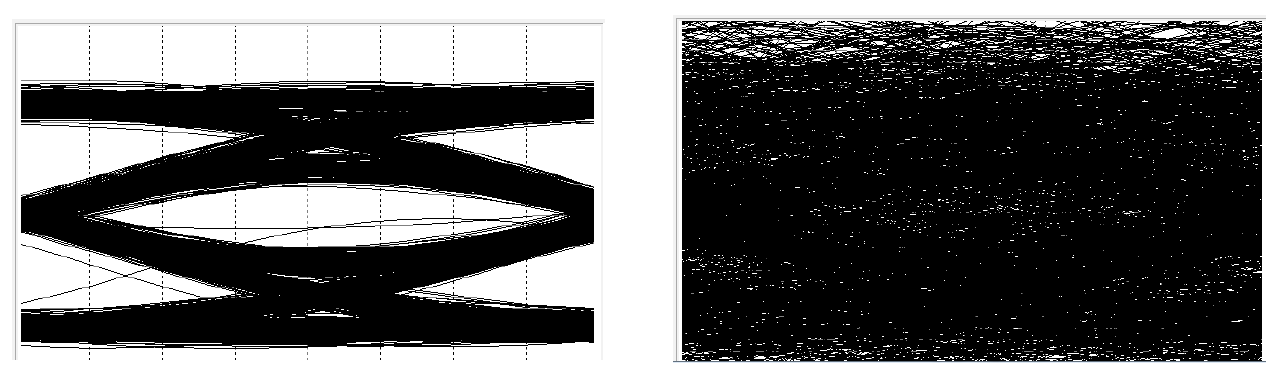
\includegraphics[width=\linewidth]{Kapitel/SIGFOX/Grafiken/sigfox_eyediagramm.png}
\captionof{figure}{Augendiagramm nicht kodiert (links), kodiert (rechts)}
\end{Figure}

LPWAN (Low Power Wide Area Network) beschreibt dann den netzwerkartigen Aufbau der über Ultra Narrow Band verbundenen Geräte, welche über auf freien ISM-Bändern genutzt werden. Die Abdeckung dieser als LPWAN bezeichneten Verbund von Netzwerkprotokollen ist allerdings sehr gering und wird erst durch SIGFOX in Europa etabliert.~\cite{sigfox.4}


\subsection*{Einsatz}
Die Einsatzgebiete von SIGFOX erstrecken sich über alle Gebiete in denen sich elektronische Geräte etabliert haben. Hervorzuhebende Sparten sind dabei die Vernetzung von Städten (Abfalleimer, Auslastungen von Straßen, …), die Vernetzung von Wohnraum (Stromverbrauch, Regelmäßigkeit des Lüftens, ….) und auch in der Gesundheitsbranche (Herzschrittmacher, Gesundheitstracker, …). Diese benannten Einsatzgebieten sind vor allem von Business zu Business relevant. Für den Heimgebrauch sind Anwendungsfälle wie das Tracken von Haustieren, die Sicherheit des eigenen Autos oder auch die Energieeffizienz im Haushalt relevant. Der Preis für die Konnektivität eine Gerätes per SIGFOX Technik zum Internet beläuft sich dabei auf 15 Euro pro Jahr und pro Gerät.

Verfügbar ist SIFOX im Moment nur in den EU Staaten Frankreich, Spanien, Niederlande und Großbritannien, wird aber in vielen weiteren Ländern und Kontinenten bereits getestet.~\cite{sigfox.2}


\subsection*{Anbieter und Gremien}

SIGFOX Anbieter sind Länderspezifisch. In Großbritannien ist arqiva, in Frankreich SIGFOX, in Spanien abertis telecom und in den Niederlanden aerea der jeweilige Anbieter der SIGFOX Technologie. Mit steigender Zahl unterstützter Länder steigt aber natürlich auch die Anzahl der Anbieter.~\cite{sigfox.1}

\subsection*{Ausblick}

Da SIGFOX noch in einem Anfangsstadium sich befindet und gerade expandiert ist die Zukunft für diese Technologie schwer vorhersehbar. Allerdings ist das Potenzial hoch und es wird unermüdlich an einer Verbesserung in Hinsicht auf Kosten, Reichweite und Energieverbrauch gearbeitet.~\cite{sigfox.3}

Die Tragweite des Internet der Dinge erscheint zumindest schwer abschätzbar hoch. Dies belegen Zahlen von den größten Global Playern der Internettechnologie. Google hat Nest, ein aufsteigendes Unternehmen für das IoT für 3,2 Milliarden US-Dollar aufgekauft. CISCO hat sich sogar an eine Schätzung gewagt und sieht im IoT einen "Wert" von 19 Billionen US-Dollar. Samsung wiederum bestätigt diese hohen Zahlen in Form von Schätzungen zu verbundenen Geräten im Jahr 2020. Diese sollen von heute (20 Millionen Geräte) auf bis zu 1,5 Milliarden Geräten im Jahr 2020 steigen.~\cite{sigfox.3}


\end{multicols}
\newpage
\section*{Historische Entwicklung}
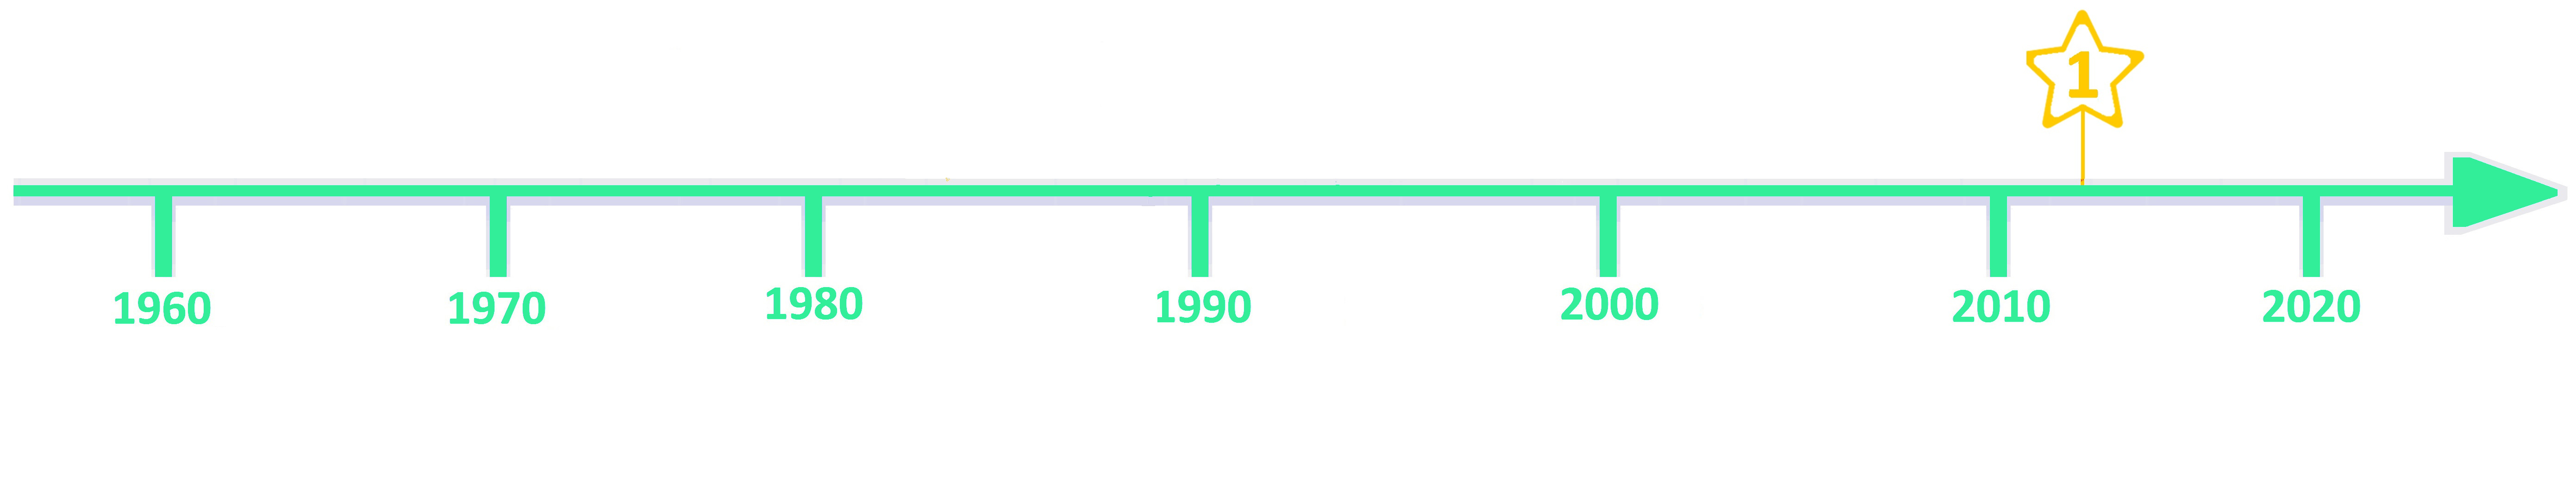
\includegraphics[width=\textwidth]{Kapitel/SIGFOX/Grafiken/Zeitstrahl}
\par
\noindent
\rowcolors{2}{}{\topicolor!20}
\begin{tabular}{p{0.5 cm}p{1.5 cm}p{15.55 cm}}
	Nr. & Datum & Entwicklungsschritte\\
	1 & 2012 & Entwicklung der SIGFOX Technologie.\\
\end{tabular}
\par
\begin{multicols}{3}

\printbibliography[segment=16,heading=subbibliography]
\end{multicols}

%~\cite{sigfox.3}

\newpage
